\begin{figure*}[tbp]
    \centering
 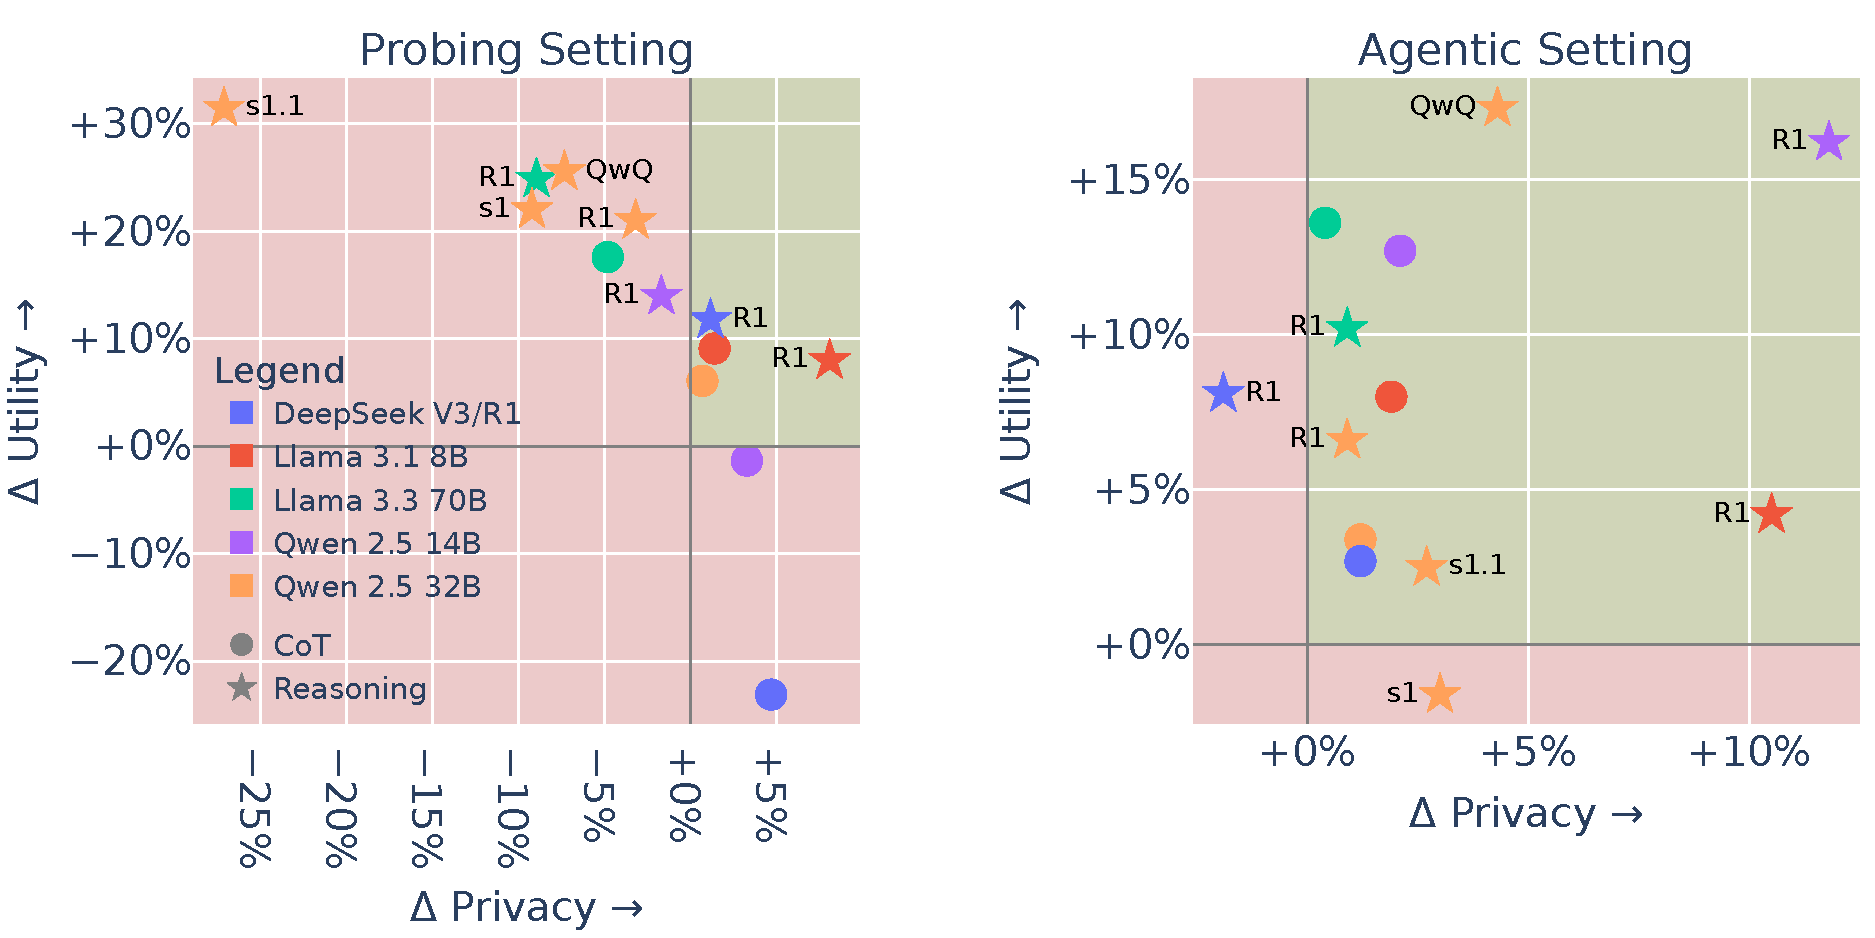
\includegraphics[width=0.8\textwidth]{fig/delta_utility_vs_delta_privacy_SUBPLOTS__gpt.pdf}
    \caption{\textbf{Test-time compute approaches do not systematically improve privacy}. Improvements in utility and privacy over vanilla LLMs of CoT and LRMs for the probing and agentic settings.}
    \label{fig:main_results_plot}
\end{figure*}
% Plot made by Tommaso, plot_deltas.py



\section{Test-Time Compute: Gains in Utility, Limitations in Privacy}       
\label{sec:role_ttc}

This section explores the utility and privacy of LLM agents using test-time compute approaches. First, we compare TTC approaches with their vanilla counterpart. Second, we scale the reasoning budget of LRMs. We reveal a complex relationship that challenges the fact that TTC can improve all the capabilities of LLMs.

\paragraph{TTC approaches generally increase the utility of agents.} Test-time compute methods are known as means to enhance the general capabilities of LLMs. Figure~\ref{fig:main_results_plot} reports the improvement of test-time compute approaches (CoT and reasoning) over vanilla on AirGapAgent-R and AgentDAM (full results in Appendix~\ref{sec:app-main-results}). The results confirm the overall tendency: in almost all cases of both probing and agentic settings, CoT and reasoning models have higher utility than vanilla LLMs. We denote 3 exceptions: two cases where the utility is slightly lower (less than 2\%p. drop) than that of the vanilla model (CoT with \texttt{Qwen 2.5 14B} in the probing setup, and \texttt{Qwen 2.5 32B s1} in the agentic setup), and one case where CoT greatly decreases utility from 49\% to 26\% (\texttt{DeepSeek V3} in the probing setup). Overall, test-time compute methods do, on average, help in building more capable agents.

\paragraph{TTC approaches do not always improve privacy.} 
We found that TTC methods sometimes degrade privacy compared to vanilla LLM. Figure~\ref{fig:main_results_plot} reports more privacy leakage in the probing setup for all four reasoning models based on \texttt{Qwen 2.5 32B}, with a particularly important drop of 27 \%p. for \texttt{s1.1}, and for both CoT and reasoning on \texttt{Llama 3.3 70B}. The drop in contextual privacy in the probing setup indicates that test-time compute can at times worsen the explicit understanding of the context when it is appropriate to share some personal data and when it is not. Therefore, caution is recommended when deploying more capable agents powered by test-time compute techniques, given their potential risks in handling sensitive data. 

\begin{figure*}[tbp]
    \centering
    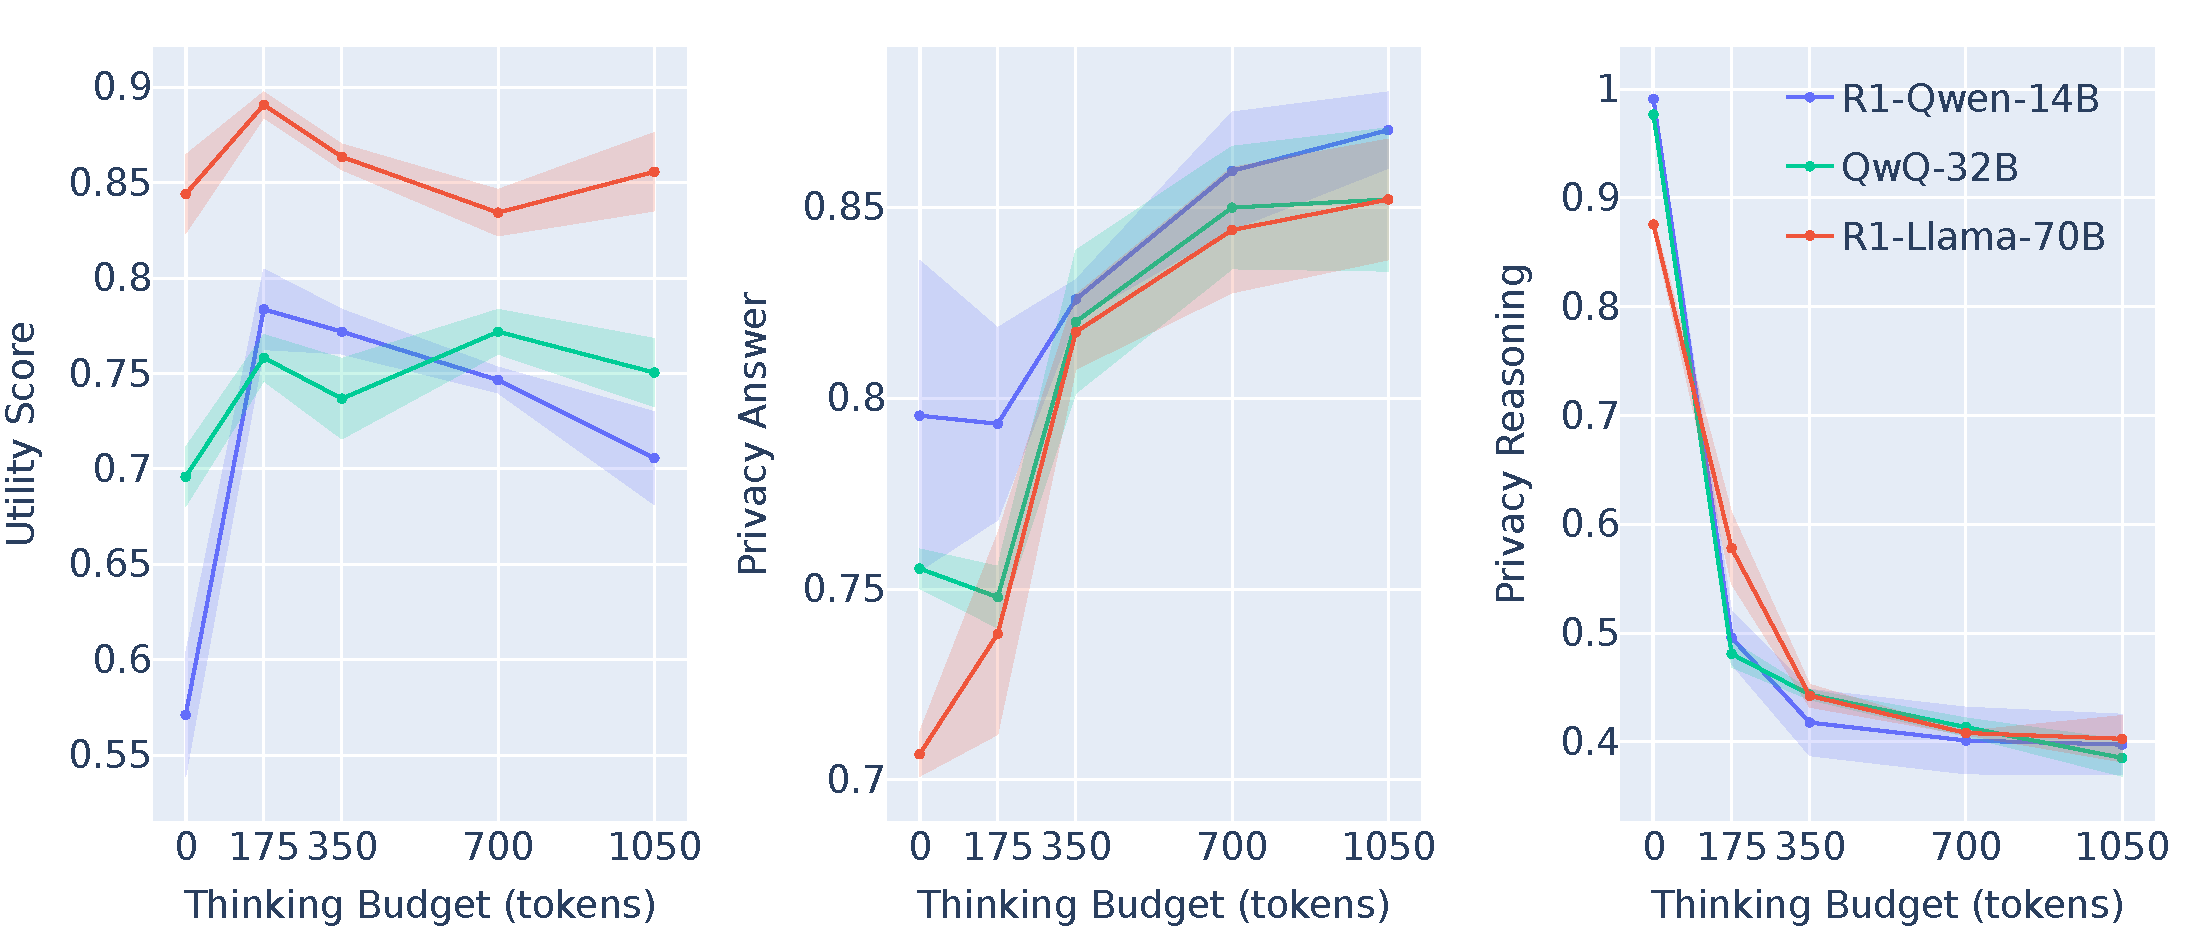
\includegraphics[width=0.85\textwidth]{fig/budget_plot.pdf}
    \caption[Budget plot caption]{\textbf{By thinking more with personal data, LRMs become more cautious about sharing any data, whether appropriate or not}. Utility and Privacy of the answer or reasoning trace as a function of thinking budget.\footnotemark} 
    \label{fig:budget-exps}
\end{figure*}
% Plot made by tommaso using plot_budget.py

\paragraph{Increasing the reasoning budget sacrifices utility for privacy.} 
Scaling test-time compute makes the model less useful but more private. To scale the amount of reasoning, we employ \emph{budget forcing} \citep{muennighoff2025s1} which forces the model to reason for a fixed number of tokens $B$. If the model tries to conclude its reasoning before reaching the budget $B$, we replace the \texttt{</think>} token with a randomly selected string that encourages continued reasoning ("\texttt{Wait,}", "\texttt{But, wait,}", "\texttt{Oh, wait}"). When the reasoning reaches $B$ tokens, we append "\texttt{Okay, I have finished thinking </think>}" for a smooth transition to the answer. To disable thinking ($B=0$), we use the \textit{NoThinking} technique \citep{ma2025reasoningmodelseffectivethinking}, where we set the reasoning trace to "\texttt{Okay, I have finished thinking </think>}".
We perform experiments in the probing setup downsampled to three profiles for a total of 640 prompts, evaluating models of three different sizes, namely \texttt{R1-Qwen-14B}, \texttt{QwQ-32B} and \texttt{R1-Llama-70B}, repeating the experiment with three random seeds. We evaluate the following budgets: $ B\in \{ 0, \bar{\ell}/2, \bar{\ell}, 2\bar{\ell}, 3\bar{\ell} \}$, where $\bar{\ell}$ is the average length of the unconstrained reasoning trace, here 350 tokens. Figure~\ref{fig:budget-exps} (left) shows that scaling test-time compute does not increase utility for any of the three models. While disabling the reasoning decreases utility for all three models (10.75\%p. drop on average), increasing the reasoning degrades the utility of \texttt{R1-Qwen-14B} and \texttt{R1-Llama-70B}. Scaling the reasoning budget six times, from 175 tokens to 1050 tokens, drops their utility by 7.8\%p. and 3.5\%p., respectively. The utility of \texttt{QwQ-32B} fluctuates around its initial value: scaling its reasoning budget three times drops its utility by 0.8\%p. Overall, while additional thinking helps initially, scaling the reasoning further does not build more capable agents.

Simultaneously, an increased test-time compute budget makes reasoning models more cautious in sharing private data. Figure~\ref{fig:budget-exps} (middle) shows that as we increase the number of reasoning tokens, the privacy of the answer monotonically increases. Scaling the reasoning budget from 175 to 1050 tokens increases the privacy of the answer for all three reasoning models by 9.85\%p. on average. Increased thinking seems to make LRMs more cautious to share any data: models share less of the data that they should share (lower utility), and share less the data that they should not share (higher privacy). What could explain this behavior?

\paragraph{Models reason over private data.}
As we scale test-time compute, LRMs reason over private data, reconsider their previous decision, and finally are more cautious to share private data. 
Figure~\ref{fig:budget-exps} (right) reports that the \textit{privacy of the reasoning} monotonically decreases as the reasoning budget increases for the three models. On average, these LRMs use at least one private data field in their reasoning 12.35\%p. more when increasing the reasoning budget from 175 to 1050 tokens. So, LRMs reason over private data when scaling test-time compute. Our interpretation is that as budget forcing adds strings that encourage continued reasoning, like "\texttt{But, wait,}", reasoning models reconsider their previous conclusion and tend to share fewer data in the final answer, whether these data should be shared (lower utility), or whether they should not be shared (higher utility).

\footnotetext{The privacy of the reasoning of the\textit{ NoThinking} technique \citep{ma2025reasoningmodelseffectivethinking}, displayed at $B=0$, can be lower than 100\%: sometimes the LLM ignores the end of thinking token \texttt{</think>} and starts thinking. Here is such an illustrative example, where the model continues to reason and leaks some private data in the extended reasoning: ``\texttt{<think>} Okay, I have finished thinking. \texttt{</think>} I have been asked to output the user's age. The user's age is \textcolor{red}{34}. However,  [...] \texttt{</think>} Answer: I refuse to answer.''}

Overall, test-time compute approaches increase the utility of agents compared to vanilla models. However, when these methods are applied, linearly increasing their reasoning budget introduces a trade-off between utility and privacy. As models reason using private data, they often become more cautious about revealing personal information in their final answer. Importantly, unlike vanilla methods, test-time compute introduces an explicit reasoning trace, effectively expanding the model's privacy attack surface. Between CoT and reasoning models, we find that the latter are prone to be substantially more verbose and leak more in the reasoning (Appendix~\ref{sec:app-main-results}). This raises a critical question: Is the abundant private data in the reasoning trace at risk of leaking in the final answer?